 

 
\subsection{Función Solver Set Bnd }
 \subsubsection{Compilación hecha con gcc en opción o0}
Se evaluó el código en assembler con instrucciones SIMD, llamado ASM, y código C de la función Solver Set Bnd sobre seis tamaños distintos de matrices: 16x16, 32x32, 64x64, 128x128, 256x256 y 512x512. Empezamos restringiéndonos a tamaños 16x16 y 512x512 de manera que si observamos tendencia evitaremos evaluar todos los tamaños con todas las variaciones de parámetros. Al variar parámetro $b$, valores de 1, 2, 3 y 10, se obtienen promedios similares en caso de matriz con tamaño 512x512 (ver Cuadro 1), alrededor de 50000 ticks para código C, sacando outliers. En caso de implementación ASM se siente levemente mayor gasto con $b$ mayor a 2 y menor gasto con $b$ igual a 1 y 2, aunque se mantiene alrededor de los 16000 ticks, menor a los de C. El desvío estandar en caso C supera los 3000 ticks y para ASM supera los 1000 ticks, levemente dispersos alrededor de la media en ambos casos. Con esto, y el porcentaje de datos con el que se promedió (columna $\%$), tomamos al promedio como representante de la mayoría de las muestras.\\
Repetimos escenario con matriz de tamaño 16x16, variando $b$ en mismos valores que para tamaño 512x512. Aunque se nota 
variación de tiempos entre mediciones no se nota gran cambio en los resultados, manteniendose el promedio de tiempos C alrededor de 1800 ticks, con desvío estandar arriba de 100 ticks, tiempos ASM alrededor de 350 ticks, con leve variación, igual que para caso 512x512 a causa de distintas variantes de $b$, y desvío estandar alrededor de 50 ticks para ASM.
Se observa en caso de 16x16 que para distintos valores de $b$ la proporción de gasto temporal de código C se mantiene en 
seis veces el gasto que tiene código ASM. A causa de esta tendencia decidimos fijar $b$ en 1 y evaluar en todos los tamaños propuestos a la función. 
\newline


\begin{table}[htbp]
\begin{center}
\begin{tabular}{|l|l|l|l|l|l|l|}
\hline
  & C & $\%$ &  SD(C)  & ASM & $\%$  & SD(ASM)\\
\hline \hline
$solver\_set\_bnd\_100\_16\_b1$ & 1728.802  & 96 &176.465  & 308.638  & 94 & 51.883 \\ \hline
$solver\_set\_bnd\_100\_16\_b2$  & 1766.234 & 98 & 203.315  &  313.909  & 88 & 13.749 \\ \hline
$solver\_set\_bnd\_100\_16\_b3$  & 1838.315  & 92 &133.411  & 388.340  & 94 & 66.619  \\ \hline
$solver\_set\_bnd\_100\_16\_b4$  & 1746.914  & 94 & 115.583  & 399.156  &  96 & 78.437 \\ 
\hline \hline
$solver\_set\_bnd\_100\_512\_b1$  & 50553.760  & 75 &7963.533   & 15610.465  & 73 &1270.874  \\ \hline

$solver\_set\_bnd\_100\_512\_b2$  & 45526.361  & 83 & 3697.485  & 15732.926  & 82 & 1622.451  \\ \hline

$solver\_set\_bnd\_100\_512\_b3$  &   51947.550  & 80 & 4330.216  & 17793.384  &78 & 1225.667 \\ \hline

$solver\_set\_bnd\_100\_512\_b4$  & 49148.481  & 83 & 3601.135   & 17413.631 & 76 & 1530.499 \\ \hline

\end{tabular}
\caption{Tabla de promedios de función Solver Set Bnd para tamaños 16x16 y 512x512. Columna $\%$ es porcentaje de datos (no outlier) con que se promedió. SD es desviación estandar.}
%\label{tabla:sencilla}
\end{center}
\end{table}

Se muestra en Figura 2$(a)$ promedio de ticks gastado en ejecución de los códigos, donde para cada tamaño los códigos se ejecutaron 100 veces.
%\begin{figure}[h]

%\centering
%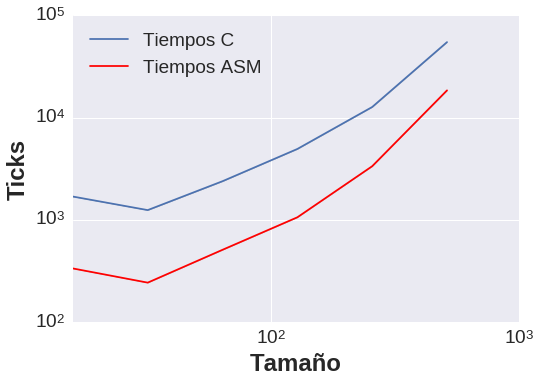
\includegraphics[scale=0.6] {solver_set_bnd_0}
  
 %\caption{Tiempos en ticks de ejecución de código C vs código ASM para función solver set bnd y gcc en opción o0.}
%\end{figure} 

\begin{figure}[htbp]
\centering

\subfigure[Compilación hecha con gcc en opción o0]{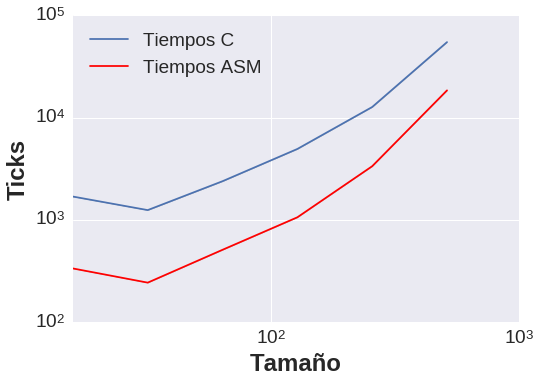
\includegraphics[width=130mm]{solver_set_bnd_0}}
\subfigure[Compilación hecha con gcc en opción o1]{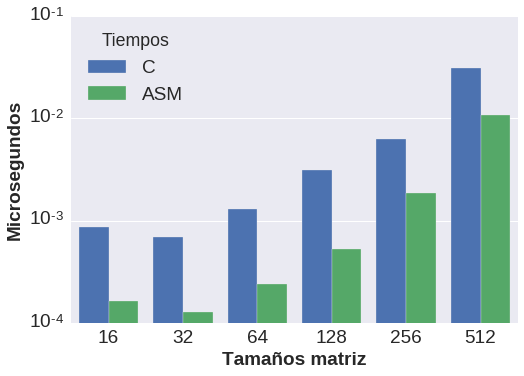
\includegraphics[width=70mm]{solver_set_bnd_1}}
\subfigure[Compilación hecha con gcc en opción o3]{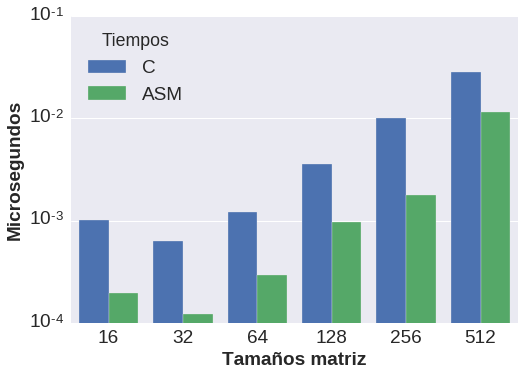
\includegraphics[width=70mm]{solver_set_bnd_3}} 

\caption{Tiempos en ticks de ejecución de código C vs código ASM para función Solver Set Bnd.} \label{fig:lego}
\end{figure}

Se ve que el código C gasta más tiempo que código ASM, achicándose esta diferencia a medida que aumenta el tamaño de matriz. Suponemos que esta ventaja de ASM sobre C se debe al uso de instrucciones SIMD en código ASM.

\subsubsection{Compilación hecha con gcc en opción o1}
Repetimos parámetros de función ($b$ en 1) para poder comparar las gráficas. El resultado se observa en Figura 2$(b)$.
%\begin{figure}[h]

%\centering
%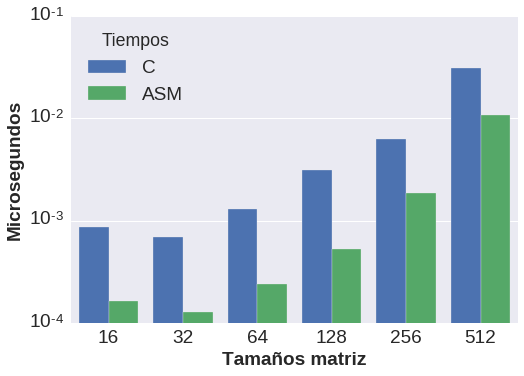
\includegraphics[scale=0.6] {solver_set_bnd_1}
  
% \caption{Tiempos en ticks de ejecución de código C vs código ASM para función solver set bnd y gcc en opción o1.}
%\end{figure} 
No se nota mejora en tiempos C, ambas gráficas, la de Solver Set Bnd y gcc o0 junto a la de Solver Set Bnd y gcc o1, muestran comportamientos similares. Tal vez observe algo en siguiente opción de optimización.



\subsubsection{Compilación hecha con gcc en opción o3}
Usamos mismas opciones de $b$ que para anteriores mediciones, $b$ en 1. El resultado se muestra en Figura 2$(c)$.
%\begin{figure}[h]

%\centering
%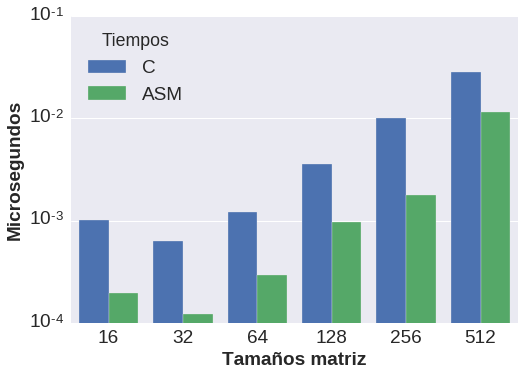
\includegraphics[scale=0.6] {solver_set_bnd_3}
  
% \caption{Tiempos en ticks de ejecución de código C vs código ASM para función solver set bnd y gcc en opción o3.}
%\end{figure} 
No vemos mejora en tiempos C, variando apenas los tiempos de este código a favor y en contra. 

\subsection{Función Solver Lin Solve}

\subsubsection{Compilación hecha con gcc en opción o0}
En este caso hemos variado los parámetros $a,b$ y $c$ solamente para tamaños de matriz 16x16 y 512x512. En la tabla siguiente se muestran los promedios obtenidos sobre datos sin outliers para valores de: $a = 1.0 $, $b$ = 1 y $c = 4.0$, llamado $1erOp$, $a = 0.3$, $b$ = 2 y $c = 2.8$, llamado $2daOp$, $a = 100.0$, $b$ = 3, $c = 20.0$ llamado $3raOp$, $a = -10.0$, $b$ = 10, $c = 0.02$, llamado $4taOp$. 
Observamos los resultados en Cuadro 2.
Para tamaño 16x16 observamos que se destaca el caso $1erOp$, donde porcentaje de datos no outliers es del 49$\%$ pero observando la gráfica de los datos (no incluída) vemos que el 61$\%$ restante se reparte un 30$\%$ arriba y otro 30$\%$ abajo de los no outliers, y por lo tanto este 49$\%$ refleja el comportamiento de la mayoría de los datos. Por otra parte en caso $2daOp$ se observa pobre ventaja de código ASM, de alrededor del 10$\%$, sobre código C, mientras que en los otros casos se obtiene un porcentaje de ventaja a favor de ASM levemente mayor. Observando el desvío estandar, datos poco dispersos respecto a la media, y el porcentaje de datos promediados (no outliers), arriba del 60$\%$ para tiempos ASM y C, salvo caso señalado antes, decidimos aceptar al promedio como representación de la mayoría de los datos. Se observa misma situación para 512x512 que para 16x16, con pobre ventaja para caso $2daOp$. A causa de esto hemos decidido evaluar la función usando $2daOp$, y las matrices $solver\rightarrow u$, $solver\rightarrow v$ para todos los tamaños propuestos: 16x16, 32x32, 64x64, 128x128, 256x256 y 512x512.
  
\begin{table}[htbp]
\begin{center}
\begin{tabular}{|l|l|l|l|l|l|l|}
\hline
  & C & $\%$ &  SD(C)  & ASM & $\%$  & SD(ASM)\\
\hline \hline
$solver\_lin\_solve\_1erOp\_16$ & 431840.428 & 49 & 5446.690 &  259397.065 & 61 &  1418.848\\ \hline

$solver\_lin\_solve\_2daOp\_16$ &  311493.016 & 59 & 2738.276 &  288969.463 & 97 & 10882.715 \\ \hline

$solver\_lin\_solve\_3raOp\_16$ & 246369.493 & 75 & 1750.180  & 203057.562 & 96 & 9578.348 \\ \hline

$solver\_lin\_solve\_4taOp\_16$ & 211043.814 & 97 & 9477.334 &  149839.649 & 97 & 3777.415\\ \hline

 
\hline \hline 


$solver\_lin\_solve\_1erOp\_512$ &  2.345*e+08  & 83 & 4.538*e+06  & 1.627*e+08 & 76 & 2.517*e+06\\ \hline

$solver\_lin\_solve\_2daOp\_512$ & 2.546*e+08  & 70 & 2.528*e+06  & 2.153*e+08 & 89 &  2.895*e+06\\ \hline

$solver\_lin\_solve\_3raOp\_512$ & 2.401*e+08 & 62 &  2.779*e+06 & 1.571*e+08 & 75 &  5.485*e+05\\ \hline

$solver\_lin\_solve\_4taOp\_512$ & 2.326*e+08 & 80 & 2.384*e+06 &  1.586*e+08 & 86 & 1.889*e+06\\ \hline

\end{tabular}
\caption{Tabla de promedios ticks función Solver Lin Solve para tamaños 16x16 y 512x512. Valores con exponente fueron redondeados para mostrarse en tabla.}
%\label{tabla:sencilla}
\end{center}
\end{table}
Con estos parámetros variamos el tamaño de las matrices y graficamos los tiempos (ver Figura 3$(a)$).
%\begin{figure}[h]

%\centering
%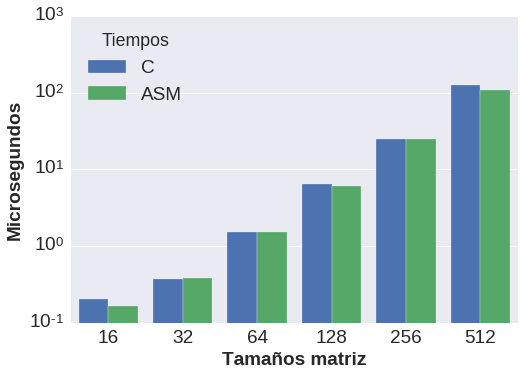
\includegraphics[scale=0.6] {solver_lin_solve_0}
  
 %\caption{Tiempos en ticks de ejecución de código C vs código ASM para función solver lin solve y gcc en opción o0.}
%\end{figure} 

\begin{figure}[htbp]
\centering

\subfigure[Compilación hecha con gcc en opción o0]{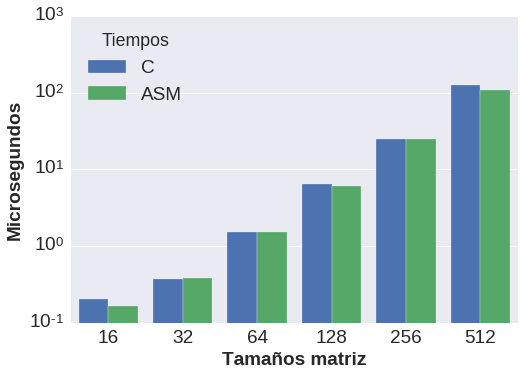
\includegraphics[width=130mm]{solver_lin_solve_0}}
\subfigure[Compilación hecha con gcc en opción o1]{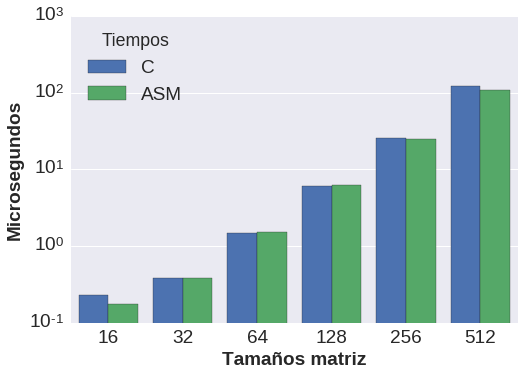
\includegraphics[width=70mm]{solver_lin_solve_1}}
\subfigure[Compilación hecha con gcc en opción o3]{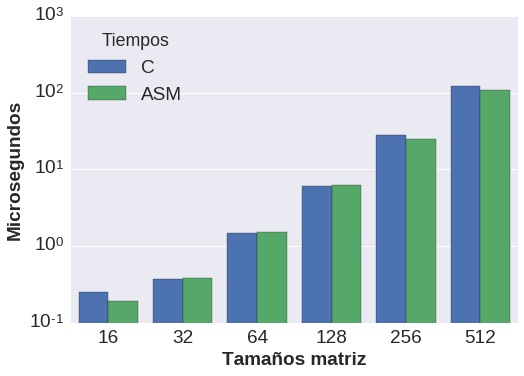
\includegraphics[width=70mm]{solver_lin_solve_3}} 

\caption{Tiempos en ticks de ejecución de código C vs código ASM para función Solver Lin Solve.} \label{fig:lego}
\end{figure}

Se observa comportamiento similar de gasto temporal, con código C apenas gastando más ticks en tamaños arriba de 128x128 que ASM.
Suponemos que este comportamiento parejo es a causa de que si bien se usa instrucciones SIMD en código ASM no se aprovecha del todo el proceso de datos en paralelo a causa de restricciones de código C de la función, que es la fuente de implementación ASM.


\subsubsection{Compilación hecha con gcc en opción o1}
Para comparar gráficas hemos decidido repetir las mediciones con los mismos parámetros que usamos en anterior medición ($a, b$ y $c$ de $2daOp$). El resultado se ve en Figura 3(b).
%\begin{figure}[h]

%\centering
%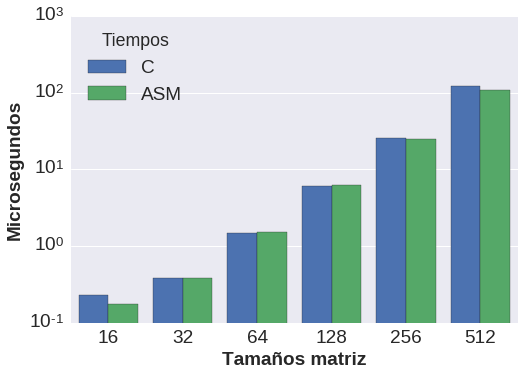
\includegraphics[scale=0.6] {solver_lin_solve_1}
  
 %\caption{Tiempos en ticks de ejecución de código C vs código ASM para función solver lin solve y gcc en opción o1.}
%\end{figure} 
No se ve una gran diferencia en los tiempos C y ASM manteniendose el comportamiento similar de gasto temporal al crecer en tamaño las matrices que usa la función.
  
\subsubsection{Compilación hecha con gcc en opción o3}
Repetimos parámetros de la función y graficamos los tiempos para distintos tamaños (Figura 3(c)).
%\begin{figure}[h]

%\centering
%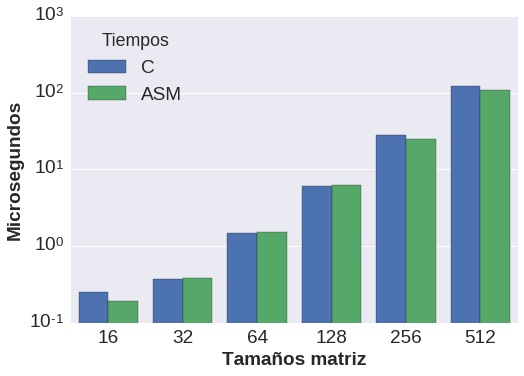
\includegraphics[scale=0.6] {solver_lin_solve_3}
  
% \caption{Tiempos en ticks de ejecución de código C vs código ASM para función solver lin solve y gcc en opción o3.}
%\end{figure} 
Se ve que no hay cambios respecto a gráfica hecha con gcc en opción o0 y o1. 

\subsection{Función Solver Project}

\subsubsection{Compilación hecha con gcc en opción o0}
Hemos medido la función variando parámetros sobre cuatro matrices diferentes: $1erOp$ que comienza con valor (0.1, 0.2) en posición (0, 0) y luego a medida que avanzamos en posiciones se incrementa en uno el valor en posición anterior y se asigna ese resultado a posición actual, $2daOp$ con mismo proceso pero comenzando en (0.2, -100), $3eraOp$ comenzando en (-10, 0.08) y $4taOp$ comenzando en (1000, 2000). Se evalúan matrices con tamaño 16x16 y 512x512 para observar si hay gran cambio en las proporciones de tiempo al ejecutar código. Se observa en Cuadro 3 los resultados y se ve que para tamaño 16x16 implementación C tiende a gastar alrededor de 50$\%$ más de clocks que código ASM.
El desvío estandar nos informa que los datos se mantienen cercanos a la media, y esto, junto a el porcentaje de datos no outliers obtenido (columna $\%$ en tabla), arriba del 60$\%$, nos da confianza de tomar al promedio como representante de datos. En caso 512x512 se observa que C también tiende a gastar arriba de 60$\%$ más del total que gasta ASM. El porcentaje de datos y el desvío estandar muestran comportamiento similar a caso 16x16. 
  
\begin{table}[htbp]
\begin{center}
\begin{tabular}{|l|l|l|l|l|l|l|}
\hline
  & C & $\%$ &  SD(C)  & ASM & $\%$  & SD(ASM)\\
\hline \hline

$solver\_project\_1erOp\_16$ & 482456.163 & 98 & 52047.911 & 258971.321 & 56 & 8276.058\\ \hline
$solver\_project\_2daOp\_16$ & 336402.153 & 98 &  19380.540  & 193437.0422 & 71 & 1054.726\\ \hline
 

$solver\_project\_3eraOp\_16$ & 276677.958 & 96 & 9241.531 & 167878.729 & 96 & 4952.023\\ \hline

$solver\_project\_4taOp\_16$ & 219557.092 & 97 &  15180.296     & 138860.719 & 89 &  2197.845\\ \hline
\hline \hline
$solver\_project\_1erOp\_512$ & 2.678*e+08 & 97 &  5.046*e+06    &  1.607*e+08 & 88 &  2.629*e+06\\ \hline
 
$solver\_project\_2daOp\_512$ &2.706*e+08  & 88 &  3.492*e+06 &   1.657*e+08 & 73 &   2.377*e+06\\ \hline


$solver\_project\_3raOp\_512$ & 2.696*e+08 & 88 &   2.406*e+06   & 1.665*e+08 & 84 & 1.915*e+06\\ \hline

$solver\_project\_4taOp\_512$ & 2.697*e+08 & 93 &  2.430*e+06  &  1.649*e+08 &  91 &    2.743*e+06\\ \hline

\end{tabular}
\caption{Tabla de promedios de ticks para función Solver Project para tamaños 16x16 y 512x512. SD es desvío estandar y $\%$ es porcentaje de datos no outliers promediados. Valores con exponente fueron redondeados para mostrarse en tabla.}
%\label{tabla:sencilla}
\end{center}
\end{table}
A causa de este análisis hemos decidido usar matrices de caso $1erOp$ para evaluar la función. En la gráfica se muestran los promedios para distintos tamaños: 16x16, 32x32, 64x64, 128x128, 256x256 y 512x512 (Figura 4$(a)$).

%\begin{figure}[h]

%\centering
%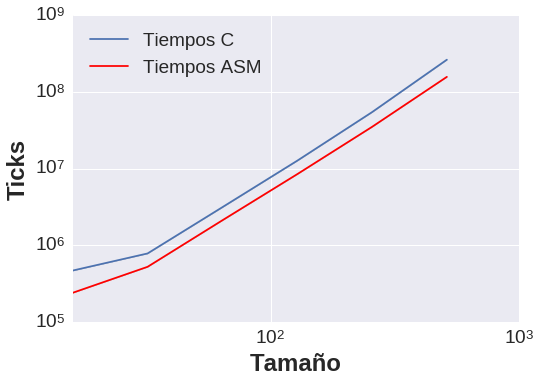
\includegraphics[scale=0.6] {solver_project_0}
 %  \caption{Tiempos en ticks de ejecución de código C vs código ASM para función solver project y gcc con opción o0}
%\end{figure}

\begin{figure}[htbp]
\centering

\subfigure[Compilación hecha con gcc en opción o0]{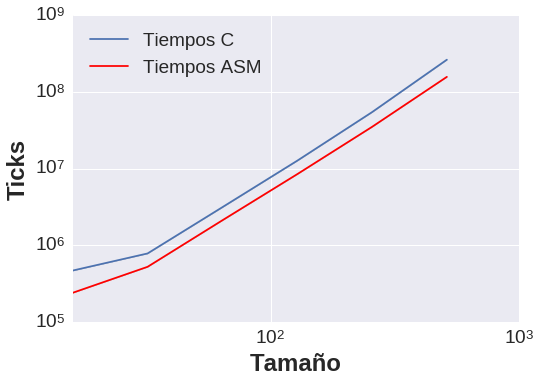
\includegraphics[width=130mm]{solver_project_0}}
\subfigure[Compilación hecha con gcc en opción o1]{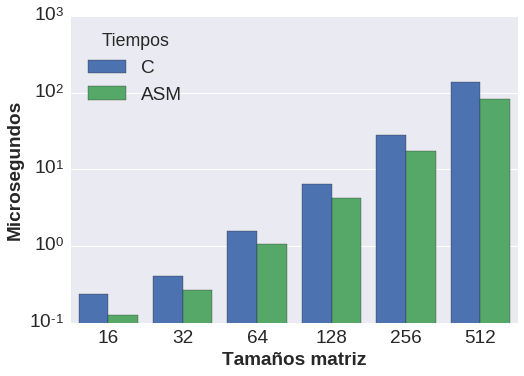
\includegraphics[width=70mm]{solver_project_1}}
\subfigure[Compilación hecha con gcc en opción o3]{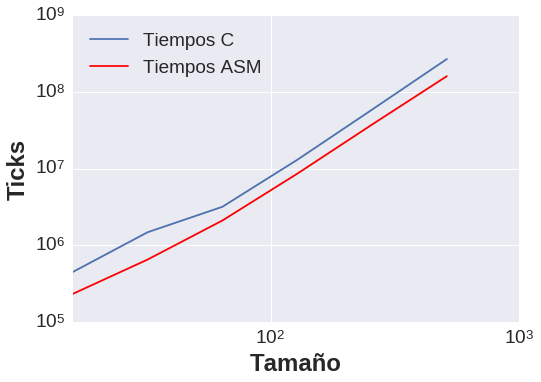
\includegraphics[width=70mm]{solver_project_3}} 

\caption{Tiempos en ticks de ejecución de código C vs código ASM para función Solver Project.} \label{fig:lego}
\end{figure}

Se observa leve ventaja de tiempos de código ASM sobre código C, creciendo ambos tiempos paralelamente. 
Suponemos que la leve ventaja que saca ejecución de un código a otro se debe a la llamada que hace Solver Project a la función Solver Lin Solve, que presentó ínfima ventaja de la implementación ASM sobre la de C.


\subsubsection{Compilación hecha con gcc en opción o1}
Se usa misma selección de parámetros que en anterior medición, matrices de caso $1erOp$. En la Figura 4$(b)$ se ve el resultado.
%\begin{figure}[h]

%\centering
%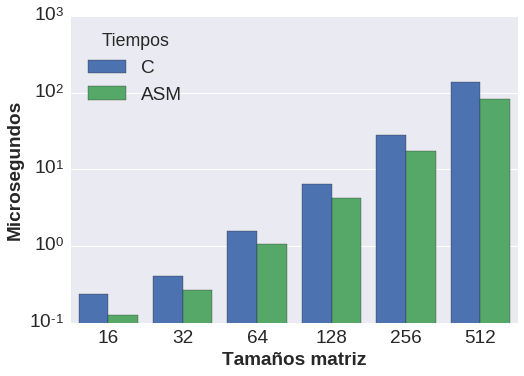
\includegraphics[scale=0.6] {solver_project_1}
 %  \caption{Tiempos en ticks de ejecución de código C vs código ASM para función solver project y gcc con opción o1}
%\end{figure}
Nuevamente no se nota cambios entre tiempos compilados con gcc opción o0 y gcc opción o1. 


\subsubsection{Compilación hecha con gcc en opción o3}
Repetimos parámetros en medición y obtuvimos el resultado de Figura 4$(c)$.
%\begin{figure}[h]

%\centering
%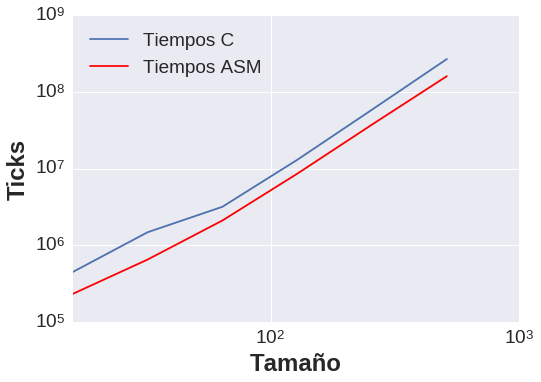
\includegraphics[scale=0.6] {solver_project_3}
 %  \caption{Tiempos en ticks de ejecución de código C vs código ASM para función solver project y gcc con opción o3}
%\end{figure}
No se nota mejora en tiempos de implementación C respecto a anteriores gráficas, la de Solver Project y gcc en o1 y la de Solver Project y gcc en o0.


